\documentclass[12pt]{beamer}
\usetheme{Warsaw}
\usepackage[utf8]{inputenc}
\usepackage[english]{babel}
\usepackage{amsmath}
\usepackage{stmaryrd}
\usepackage{amsfonts}
\usepackage{amssymb}
\usepackage{graphicx}
\usepackage{color}
\usepackage[backend=bibtex, style=authoryear, maxcitenames=2]{biblatex}
\addbibresource{../../Ausarbeitung/references.bib} 
\renewcommand*{\bibfont}{\footnotesize}
\usepackage{url}
\definecolor{lila}{RGB}{128,0,128}

\newcommand{\myCite}[1]{{\scriptsize\parencite{#1}}}

\setbeamertemplate{navigation symbols}{}
\setbeamertemplate{footline}{%
	\raisebox{5pt}{%
		\makebox[\paperwidth]{%
			\hfill\makebox[10pt]{%
				\textcolor{gray}{\footnotesize\insertframenumber}
			}
		}
	}
}

%\setbeamercovered{transparent} 
%\logo{}  
%\subject{} 
\begin{document} 
		
\begin{frame}[plain,noframenumbering]
	\begin{minipage}{0.25\textwidth}
		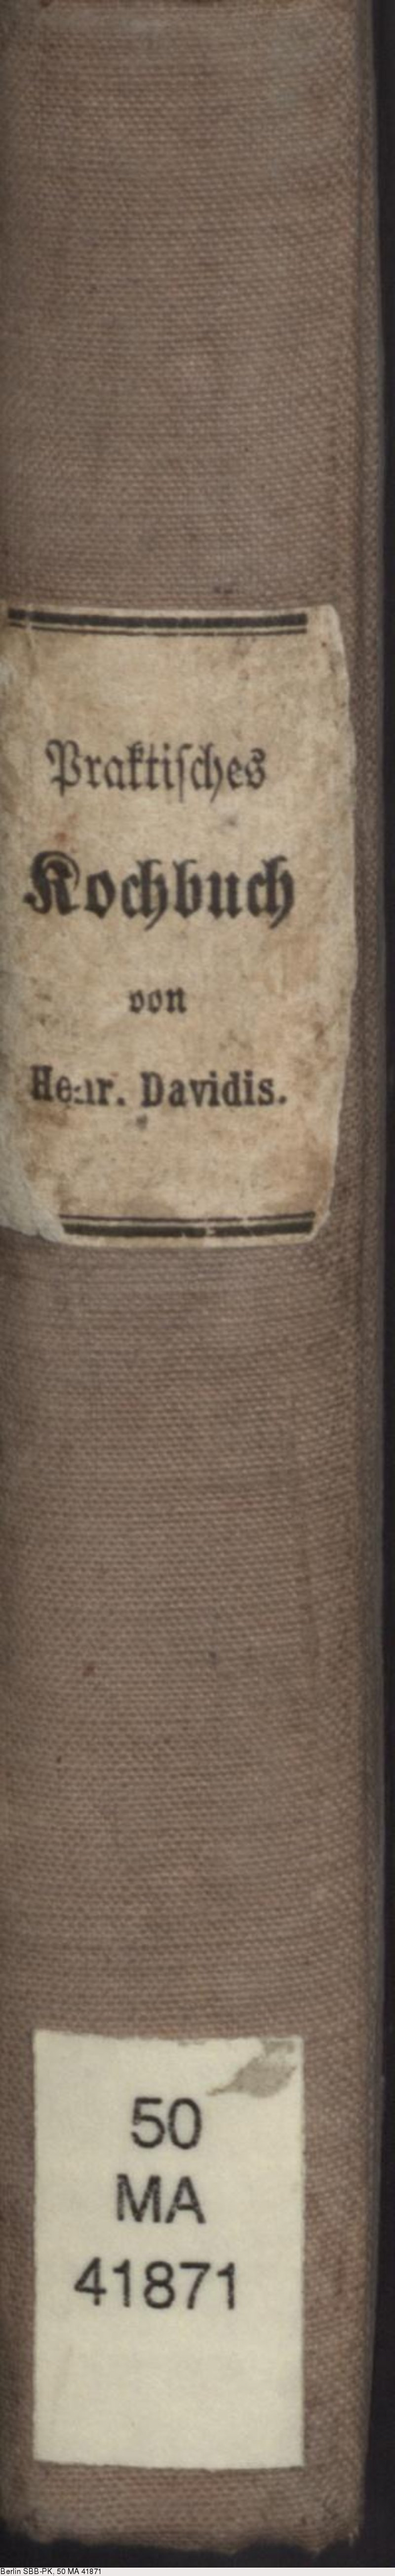
\includegraphics[scale=0.049]{Images/Buchruecken}
	\end{minipage}
	\begin{minipage}{0.7\textwidth}
		\begin{center}
			\vspace{-1.5cm}
			\Large{Extracting recipe ingredients \\ from cookbooks} \\
			\vspace{0.5cm}
			\large{Der Beginn einer Master-Arbeit} \\
			\small{von \\ \vspace{-0.1cm} Torsten Knauf}
		\end{center}
	\end{minipage}
\end{frame}

\begin{frame}
	\tableofcontents
\end{frame}

\section{Hintergrund der Arbeit}
\subsection{Was und wieso}
\begin{frame}{Was und wieso}
	\begin{itemize}
		\item Was?
		\begin{itemize}
			\item Zutaten der Rezepte automatisch extrahieren
			\item Im Sinne des Semantic Webs zur Verfügung stellen 
		\end{itemize}
		\item Wieso?
		\begin{itemize}
			\item Ernährungswissenschaften
			\item Soziologische Forschung wie z.B. Globalisierung, Wohlstand, ...
		\end{itemize}
	\end{itemize}
\end{frame}

\subsection{Digitalisierung}
\begin{frame}{Digitalisierung}
	\myCite{DTA} \\
	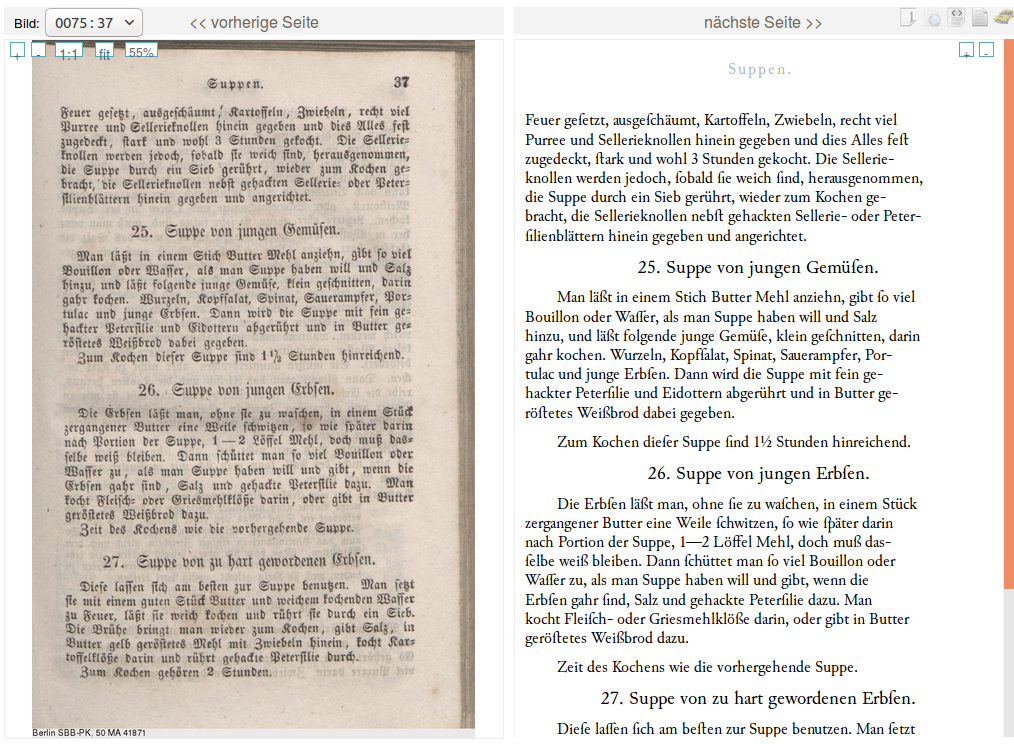
\includegraphics[scale=0.3]{Images/BeispielSeite}
\end{frame}

\begin{frame}
	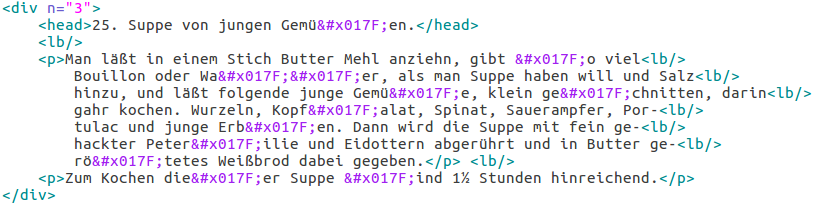
\includegraphics[scale=0.4]{Images/derenXML} \\
\end{frame}

\begin{frame}
	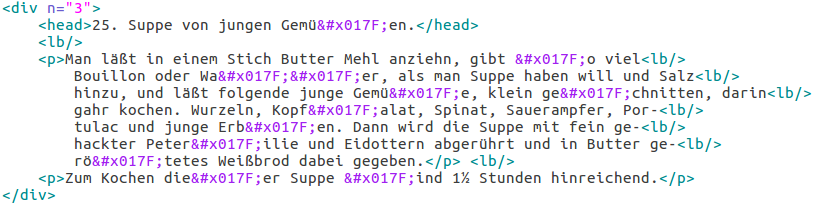
\includegraphics[scale=0.4]{Images/derenXML} \\
	\vspace{0.3cm}
	\hrulefill
	\vspace{0.3cm}
	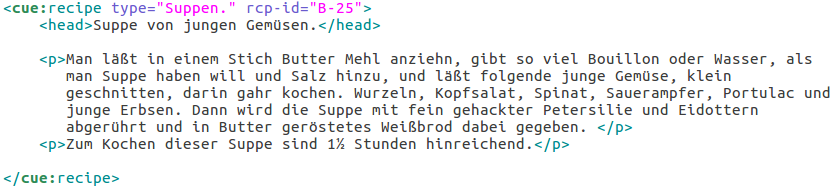
\includegraphics[scale=0.4]{Images/unserXML}
\end{frame}

\subsection{Das Tagging}
\begin{frame}{Das Tagging}
	\begin{itemize}
		\item \textbf{cueML} (culinary editions markup language)
		\begin{itemize}
			\item Erweiterung von \textbf{TEI} (Text Encoding Initiative)
			\item Erweitert mit \textbf{https://schema.org/Recipe}
		\end{itemize}
	\end{itemize}
	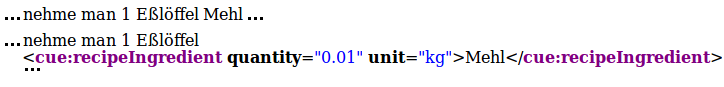
\includegraphics[scale=0.45]{Images/TagBeispiel}
\end{frame}

\begin{frame}{Das Tagging \textcolor{red}{ - Achtung}}
	\begin{itemize}
		\item Scorzoner-Wurzeln, Petersilienwurzel
		\item 8 Pfennig Weißbrot, Loth, Quart
		\item \textit{"Wie die vorhergehende, nur mit weiß gebranntem Mehl und Bouillon
			zubereitet, die Nelken bleiben weg."}
		\item \textit{"[Man] legt ihn in einen eisernen Topf, darauf 1/4 Pfund in Scheiben geschnittenen rohen Schinken oder Sommerwurst"} $\rightarrow$ \textcolor{lila}{$<$recipeIngredientAlt$>$}
		\item \textit{"Fehlt ihm die gewünschte Süße, so wird zeitig ein Stück Zucker dazu gethan, so wie beim Anrichten die Brühe mit etwas Kartoffelmehl gebunden gemacht."} \\ $\rightarrow$ \textcolor{lila}{$<$recipeOptionalIngredient$>$}
	\end{itemize}
\end{frame}


\section{Ansätze für automatisches Tagging}
\subsection{Was muss die Lösung alles können?}
\begin{frame}{Ansätze für automatisches Tagging}
	\begin{itemize}
		\item Was muss die Lösung alles können?
		\begin{itemize}
			\item \textbf{\textcolor{red}{Aus reinem Text alle Zutaten eindeutig erkennen}}
			\item Zutaten erkennen \textbf{(Lemmatisierung)} und Zuordnen der Quantitäten und Einheiten zu den entsprechenden Zutaten \textbf{(Structure prediction for NLP)}
			\item Unterscheidung ob eine Zutat verwendet werden soll, nicht verwendet werden soll, optional ist, eine Alternative ist \textbf{(Klassifizierungs-Probleme)}
			\item Verweise erkennen und verlinken \textbf{(Klassifizierungs-Probleme, Structure prediction for NLP)}
		\end{itemize}
	\end{itemize}
\end{frame}

\subsection{Bestehende Ansätze}
\begin{frame}
	\begin{itemize}
		\item Bestehende Ansätze:
		\begin{itemize}
			\item Reguläre Ausdrücke \parencite{REgutGenug}
			\item Kontextfreie Grammatik: \parencite{GrammaBased} \\
			$NP \rightarrow DT? JJ\textsuperscript{*} ING$
			\item Conditional Random Field \parencite{CRFPaper}, \parencite{CRFZeit}
		\end{itemize}
	\end{itemize}
\end{frame}

\subsection{Typischer Workflow}
\begin{frame}
	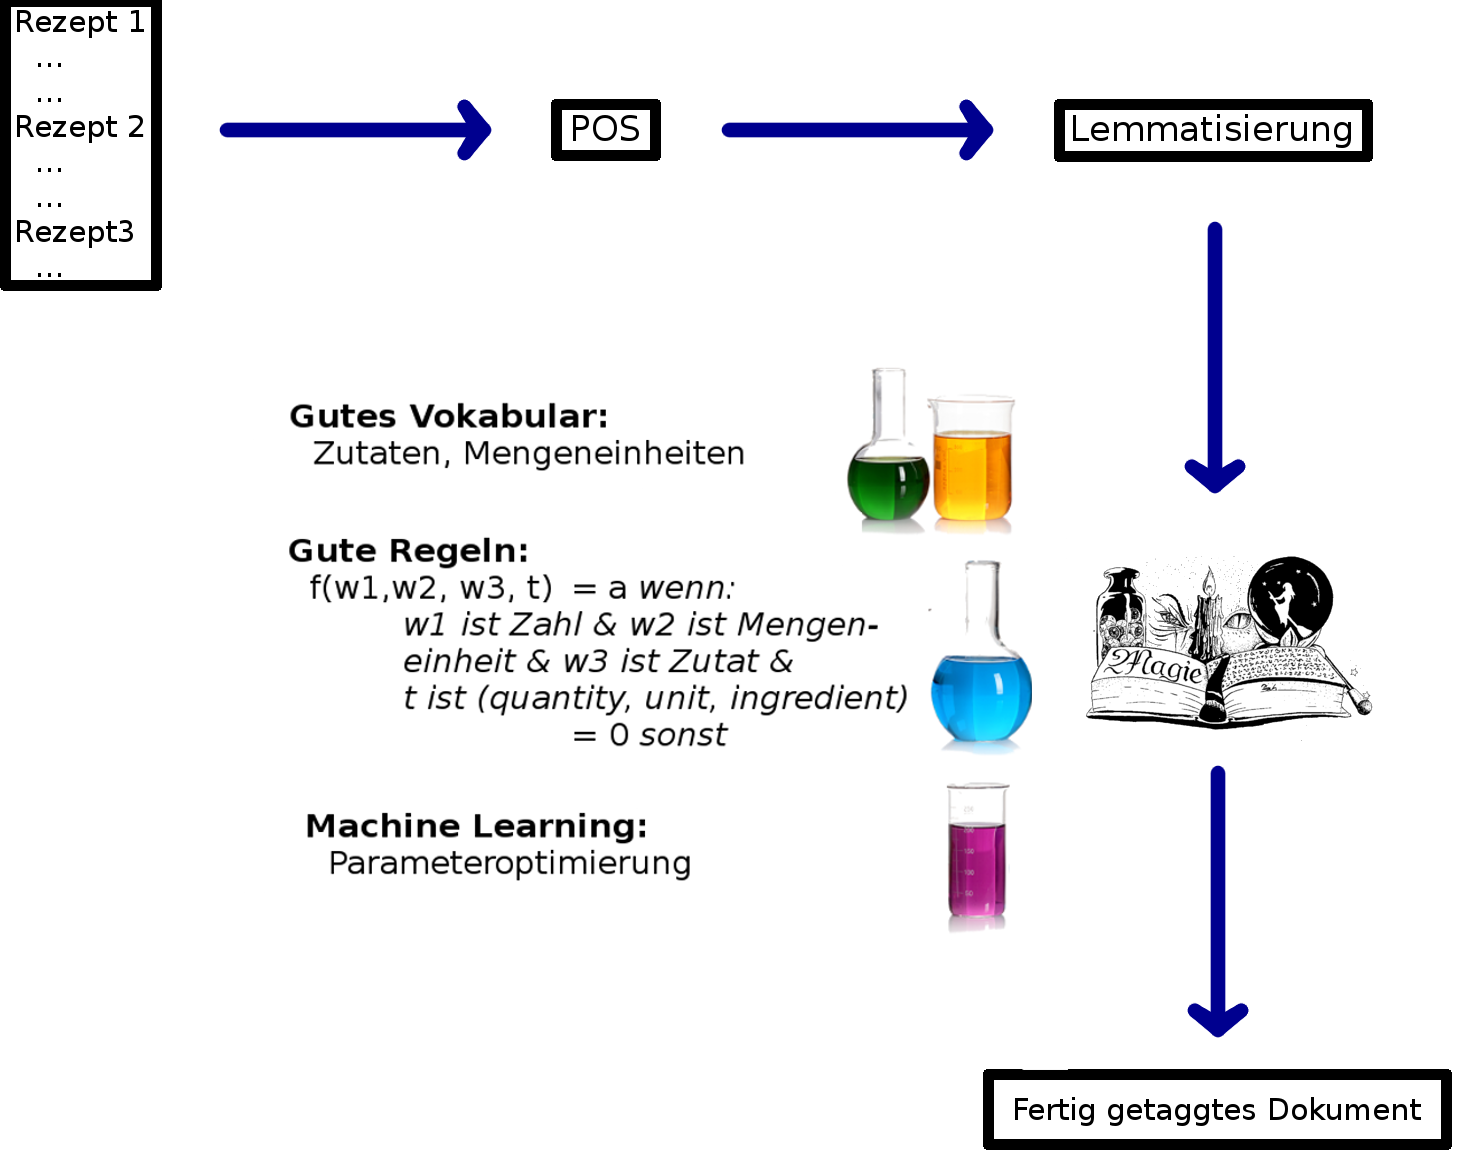
\includegraphics[scale=0.8]{Images/workflow}
\end{frame}

\begin{frame}
	\begin{center}
		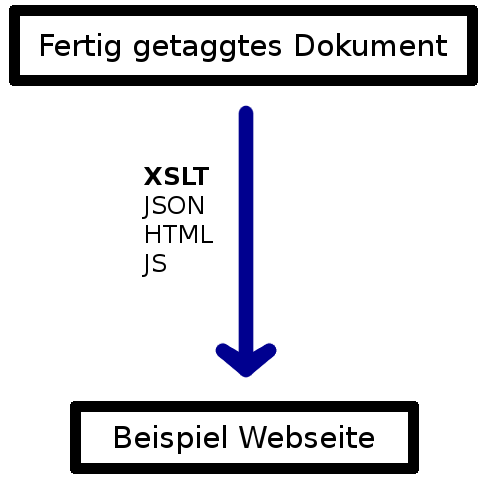
\includegraphics[scale=1]{Images/webseite}
	\end{center}
\end{frame}


\section{Literatur}
\subsection{Literatursuche ist toll}
\begin{frame}{Literatursuche ist toll}
	\textbf{\textcolor{red}{Aus reinem Text alle Zutaten eindeutig erkennen}}
	\begin{itemize}
		\item Problem verstehen $\rightarrow$ Teilgebiet vom Text Mining 
		\item Zerlegung in Teilprobleme $\rightarrow$ Structure prediction for NLP, Lemmatisierung, Klassifizierungs-Probleme, Conditional Random Field
		\item "Das Rad [nicht] neu erfinden"
		\begin{itemize}
			\item Bestehende Lösungen nutzen ist viel produktiver
			\item Mehrere unterschiedliche Lösungen / Ideen / Meinungen ergänzen sich oft
		\end{itemize}
	\end{itemize}
\end{frame}


\subsection{Literaturverzeichnis}
\begin{frame}[t,allowframebreaks]{Literaturverzeichnis}
	\printbibliography[heading=none]
\end{frame}

\end{document}